% Options for packages loaded elsewhere
% Options for packages loaded elsewhere
\PassOptionsToPackage{unicode}{hyperref}
\PassOptionsToPackage{hyphens}{url}
\PassOptionsToPackage{dvipsnames,svgnames,x11names}{xcolor}
%
\documentclass[
  letterpaper,
  DIV=11,
  numbers=noendperiod]{scrartcl}
\usepackage{xcolor}
\usepackage{amsmath,amssymb}
\setcounter{secnumdepth}{-\maxdimen} % remove section numbering
\usepackage{iftex}
\ifPDFTeX
  \usepackage[T1]{fontenc}
  \usepackage[utf8]{inputenc}
  \usepackage{textcomp} % provide euro and other symbols
\else % if luatex or xetex
  \usepackage{unicode-math} % this also loads fontspec
  \defaultfontfeatures{Scale=MatchLowercase}
  \defaultfontfeatures[\rmfamily]{Ligatures=TeX,Scale=1}
\fi
\usepackage{lmodern}
\ifPDFTeX\else
  % xetex/luatex font selection
\fi
% Use upquote if available, for straight quotes in verbatim environments
\IfFileExists{upquote.sty}{\usepackage{upquote}}{}
\IfFileExists{microtype.sty}{% use microtype if available
  \usepackage[]{microtype}
  \UseMicrotypeSet[protrusion]{basicmath} % disable protrusion for tt fonts
}{}
\makeatletter
\@ifundefined{KOMAClassName}{% if non-KOMA class
  \IfFileExists{parskip.sty}{%
    \usepackage{parskip}
  }{% else
    \setlength{\parindent}{0pt}
    \setlength{\parskip}{6pt plus 2pt minus 1pt}}
}{% if KOMA class
  \KOMAoptions{parskip=half}}
\makeatother
% Make \paragraph and \subparagraph free-standing
\makeatletter
\ifx\paragraph\undefined\else
  \let\oldparagraph\paragraph
  \renewcommand{\paragraph}{
    \@ifstar
      \xxxParagraphStar
      \xxxParagraphNoStar
  }
  \newcommand{\xxxParagraphStar}[1]{\oldparagraph*{#1}\mbox{}}
  \newcommand{\xxxParagraphNoStar}[1]{\oldparagraph{#1}\mbox{}}
\fi
\ifx\subparagraph\undefined\else
  \let\oldsubparagraph\subparagraph
  \renewcommand{\subparagraph}{
    \@ifstar
      \xxxSubParagraphStar
      \xxxSubParagraphNoStar
  }
  \newcommand{\xxxSubParagraphStar}[1]{\oldsubparagraph*{#1}\mbox{}}
  \newcommand{\xxxSubParagraphNoStar}[1]{\oldsubparagraph{#1}\mbox{}}
\fi
\makeatother

\usepackage{color}
\usepackage{fancyvrb}
\newcommand{\VerbBar}{|}
\newcommand{\VERB}{\Verb[commandchars=\\\{\}]}
\DefineVerbatimEnvironment{Highlighting}{Verbatim}{commandchars=\\\{\}}
% Add ',fontsize=\small' for more characters per line
\usepackage{framed}
\definecolor{shadecolor}{RGB}{241,243,245}
\newenvironment{Shaded}{\begin{snugshade}}{\end{snugshade}}
\newcommand{\AlertTok}[1]{\textcolor[rgb]{0.68,0.00,0.00}{#1}}
\newcommand{\AnnotationTok}[1]{\textcolor[rgb]{0.37,0.37,0.37}{#1}}
\newcommand{\AttributeTok}[1]{\textcolor[rgb]{0.40,0.45,0.13}{#1}}
\newcommand{\BaseNTok}[1]{\textcolor[rgb]{0.68,0.00,0.00}{#1}}
\newcommand{\BuiltInTok}[1]{\textcolor[rgb]{0.00,0.23,0.31}{#1}}
\newcommand{\CharTok}[1]{\textcolor[rgb]{0.13,0.47,0.30}{#1}}
\newcommand{\CommentTok}[1]{\textcolor[rgb]{0.37,0.37,0.37}{#1}}
\newcommand{\CommentVarTok}[1]{\textcolor[rgb]{0.37,0.37,0.37}{\textit{#1}}}
\newcommand{\ConstantTok}[1]{\textcolor[rgb]{0.56,0.35,0.01}{#1}}
\newcommand{\ControlFlowTok}[1]{\textcolor[rgb]{0.00,0.23,0.31}{\textbf{#1}}}
\newcommand{\DataTypeTok}[1]{\textcolor[rgb]{0.68,0.00,0.00}{#1}}
\newcommand{\DecValTok}[1]{\textcolor[rgb]{0.68,0.00,0.00}{#1}}
\newcommand{\DocumentationTok}[1]{\textcolor[rgb]{0.37,0.37,0.37}{\textit{#1}}}
\newcommand{\ErrorTok}[1]{\textcolor[rgb]{0.68,0.00,0.00}{#1}}
\newcommand{\ExtensionTok}[1]{\textcolor[rgb]{0.00,0.23,0.31}{#1}}
\newcommand{\FloatTok}[1]{\textcolor[rgb]{0.68,0.00,0.00}{#1}}
\newcommand{\FunctionTok}[1]{\textcolor[rgb]{0.28,0.35,0.67}{#1}}
\newcommand{\ImportTok}[1]{\textcolor[rgb]{0.00,0.46,0.62}{#1}}
\newcommand{\InformationTok}[1]{\textcolor[rgb]{0.37,0.37,0.37}{#1}}
\newcommand{\KeywordTok}[1]{\textcolor[rgb]{0.00,0.23,0.31}{\textbf{#1}}}
\newcommand{\NormalTok}[1]{\textcolor[rgb]{0.00,0.23,0.31}{#1}}
\newcommand{\OperatorTok}[1]{\textcolor[rgb]{0.37,0.37,0.37}{#1}}
\newcommand{\OtherTok}[1]{\textcolor[rgb]{0.00,0.23,0.31}{#1}}
\newcommand{\PreprocessorTok}[1]{\textcolor[rgb]{0.68,0.00,0.00}{#1}}
\newcommand{\RegionMarkerTok}[1]{\textcolor[rgb]{0.00,0.23,0.31}{#1}}
\newcommand{\SpecialCharTok}[1]{\textcolor[rgb]{0.37,0.37,0.37}{#1}}
\newcommand{\SpecialStringTok}[1]{\textcolor[rgb]{0.13,0.47,0.30}{#1}}
\newcommand{\StringTok}[1]{\textcolor[rgb]{0.13,0.47,0.30}{#1}}
\newcommand{\VariableTok}[1]{\textcolor[rgb]{0.07,0.07,0.07}{#1}}
\newcommand{\VerbatimStringTok}[1]{\textcolor[rgb]{0.13,0.47,0.30}{#1}}
\newcommand{\WarningTok}[1]{\textcolor[rgb]{0.37,0.37,0.37}{\textit{#1}}}

\usepackage{longtable,booktabs,array}
\newcounter{none} % for unnumbered tables
\usepackage{calc} % for calculating minipage widths
% Correct order of tables after \paragraph or \subparagraph
\usepackage{etoolbox}
\makeatletter
\patchcmd\longtable{\par}{\if@noskipsec\mbox{}\fi\par}{}{}
\makeatother
% Allow footnotes in longtable head/foot
\IfFileExists{footnotehyper.sty}{\usepackage{footnotehyper}}{\usepackage{footnote}}
\makesavenoteenv{longtable}
\usepackage{graphicx}
\makeatletter
\newsavebox\pandoc@box
\newcommand*\pandocbounded[1]{% scales image to fit in text height/width
  \sbox\pandoc@box{#1}%
  \Gscale@div\@tempa{\textheight}{\dimexpr\ht\pandoc@box+\dp\pandoc@box\relax}%
  \Gscale@div\@tempb{\linewidth}{\wd\pandoc@box}%
  \ifdim\@tempb\p@<\@tempa\p@\let\@tempa\@tempb\fi% select the smaller of both
  \ifdim\@tempa\p@<\p@\scalebox{\@tempa}{\usebox\pandoc@box}%
  \else\usebox{\pandoc@box}%
  \fi%
}
% Set default figure placement to htbp
\def\fps@figure{htbp}
\makeatother





\setlength{\emergencystretch}{3em} % prevent overfull lines

\providecommand{\tightlist}{%
  \setlength{\itemsep}{0pt}\setlength{\parskip}{0pt}}



 


\KOMAoption{captions}{tableheading}
\makeatletter
\@ifpackageloaded{caption}{}{\usepackage{caption}}
\AtBeginDocument{%
\ifdefined\contentsname
  \renewcommand*\contentsname{Table of contents}
\else
  \newcommand\contentsname{Table of contents}
\fi
\ifdefined\listfigurename
  \renewcommand*\listfigurename{List of Figures}
\else
  \newcommand\listfigurename{List of Figures}
\fi
\ifdefined\listtablename
  \renewcommand*\listtablename{List of Tables}
\else
  \newcommand\listtablename{List of Tables}
\fi
\ifdefined\figurename
  \renewcommand*\figurename{Figure}
\else
  \newcommand\figurename{Figure}
\fi
\ifdefined\tablename
  \renewcommand*\tablename{Table}
\else
  \newcommand\tablename{Table}
\fi
}
\@ifpackageloaded{float}{}{\usepackage{float}}
\floatstyle{ruled}
\@ifundefined{c@chapter}{\newfloat{codelisting}{h}{lop}}{\newfloat{codelisting}{h}{lop}[chapter]}
\floatname{codelisting}{Listing}
\newcommand*\listoflistings{\listof{codelisting}{List of Listings}}
\makeatother
\makeatletter
\makeatother
\makeatletter
\@ifpackageloaded{caption}{}{\usepackage{caption}}
\@ifpackageloaded{subcaption}{}{\usepackage{subcaption}}
\makeatother
\usepackage{bookmark}
\IfFileExists{xurl.sty}{\usepackage{xurl}}{} % add URL line breaks if available
\urlstyle{same}
% fallback for those not using the hyperref driver hyperxmp:
\makeatletter
\@ifundefined{xmpquote}{\newcommand{\xmpquote}[1]{#1}}{}
\makeatother
\hypersetup{
  pdftitle={Class13: RNA-Seq analysis mini-project},
  pdfauthor={Hyuntae An (TSN: 200231511)},
  colorlinks=true,
  linkcolor={blue},
  filecolor={Maroon},
  citecolor={Blue},
  urlcolor={Blue},
  pdfcreator={LaTeX via pandoc}}


\title{Class13: RNA-Seq analysis mini-project}
\author{Hyuntae An (TSN: 200231511)}
\date{}
\begin{document}
\maketitle


\subsection{Background}\label{background}

Analysis of high-throughput biological data typically yields a list of
genes or proteins requiring further interpretation - for example the
ranked lists of differentially expressed genes we have been generating
from our RNA-seq analysis to date.

Our intention is typically to use such lists to gain novel insights
about genes and proteins that may have roles in a given phenomenon,
phenotype or disease progression. However, in many cases these `raw'
gene lists are challenging to interpret due to their large size and lack
of useful annotations. Hence, our expensively assembled gene lists often
fail to convey the full degree of possible insight about the condition
being studied.

Pathway analysis (also known as gene set analysis or over-representation
analysis), aims to reduce the complexity of interpreting gene lists via
mapping the listed genes to known (i.e.~annotated) biological pathways,
processes and functions.

\subsection{Differential Expression
Analysis}\label{differential-expression-analysis}

\begin{Shaded}
\begin{Highlighting}[]
\FunctionTok{library}\NormalTok{(DESeq2)}
\end{Highlighting}
\end{Shaded}

\begin{verbatim}
Loading required package: S4Vectors
\end{verbatim}

\begin{verbatim}
Loading required package: stats4
\end{verbatim}

\begin{verbatim}
Loading required package: BiocGenerics
\end{verbatim}

\begin{verbatim}
Loading required package: generics
\end{verbatim}

\begin{verbatim}

Attaching package: 'generics'
\end{verbatim}

\begin{verbatim}
The following objects are masked from 'package:base':

    as.difftime, as.factor, as.ordered, intersect, is.element, setdiff,
    setequal, union
\end{verbatim}

\begin{verbatim}

Attaching package: 'BiocGenerics'
\end{verbatim}

\begin{verbatim}
The following objects are masked from 'package:stats':

    IQR, mad, sd, var, xtabs
\end{verbatim}

\begin{verbatim}
The following objects are masked from 'package:base':

    anyDuplicated, aperm, append, as.data.frame, basename, cbind,
    colnames, dirname, do.call, duplicated, eval, evalq, Filter, Find,
    get, grep, grepl, is.unsorted, lapply, Map, mapply, match, mget,
    order, paste, pmax, pmax.int, pmin, pmin.int, Position, rank,
    rbind, Reduce, rownames, sapply, saveRDS, table, tapply, unique,
    unsplit, which.max, which.min
\end{verbatim}

\begin{verbatim}

Attaching package: 'S4Vectors'
\end{verbatim}

\begin{verbatim}
The following object is masked from 'package:utils':

    findMatches
\end{verbatim}

\begin{verbatim}
The following objects are masked from 'package:base':

    expand.grid, I, unname
\end{verbatim}

\begin{verbatim}
Loading required package: IRanges
\end{verbatim}

\begin{verbatim}
Loading required package: GenomicRanges
\end{verbatim}

\begin{verbatim}
Loading required package: Seqinfo
\end{verbatim}

\begin{verbatim}
Loading required package: SummarizedExperiment
\end{verbatim}

\begin{verbatim}
Loading required package: MatrixGenerics
\end{verbatim}

\begin{verbatim}
Loading required package: matrixStats
\end{verbatim}

\begin{verbatim}

Attaching package: 'MatrixGenerics'
\end{verbatim}

\begin{verbatim}
The following objects are masked from 'package:matrixStats':

    colAlls, colAnyNAs, colAnys, colAvgsPerRowSet, colCollapse,
    colCounts, colCummaxs, colCummins, colCumprods, colCumsums,
    colDiffs, colIQRDiffs, colIQRs, colLogSumExps, colMadDiffs,
    colMads, colMaxs, colMeans2, colMedians, colMins, colOrderStats,
    colProds, colQuantiles, colRanges, colRanks, colSdDiffs, colSds,
    colSums2, colTabulates, colVarDiffs, colVars, colWeightedMads,
    colWeightedMeans, colWeightedMedians, colWeightedSds,
    colWeightedVars, rowAlls, rowAnyNAs, rowAnys, rowAvgsPerColSet,
    rowCollapse, rowCounts, rowCummaxs, rowCummins, rowCumprods,
    rowCumsums, rowDiffs, rowIQRDiffs, rowIQRs, rowLogSumExps,
    rowMadDiffs, rowMads, rowMaxs, rowMeans2, rowMedians, rowMins,
    rowOrderStats, rowProds, rowQuantiles, rowRanges, rowRanks,
    rowSdDiffs, rowSds, rowSums2, rowTabulates, rowVarDiffs, rowVars,
    rowWeightedMads, rowWeightedMeans, rowWeightedMedians,
    rowWeightedSds, rowWeightedVars
\end{verbatim}

\begin{verbatim}
Loading required package: Biobase
\end{verbatim}

\begin{verbatim}
Welcome to Bioconductor

    Vignettes contain introductory material; view with
    'browseVignettes()'. To cite Bioconductor, see
    'citation("Biobase")', and for packages 'citation("pkgname")'.
\end{verbatim}

\begin{verbatim}

Attaching package: 'Biobase'
\end{verbatim}

\begin{verbatim}
The following object is masked from 'package:MatrixGenerics':

    rowMedians
\end{verbatim}

\begin{verbatim}
The following objects are masked from 'package:matrixStats':

    anyMissing, rowMedians
\end{verbatim}

\begin{Shaded}
\begin{Highlighting}[]
\NormalTok{metaFile }\OtherTok{\textless{}{-}} \StringTok{"GSE37704\_metadata.csv"}
\NormalTok{countFile }\OtherTok{\textless{}{-}} \StringTok{"GSE37704\_featurecounts.csv"}

\CommentTok{\# Import metadata and take a peek}
\NormalTok{colData }\OtherTok{=} \FunctionTok{read.csv}\NormalTok{(metaFile, }\AttributeTok{row.names=}\DecValTok{1}\NormalTok{)}
\FunctionTok{head}\NormalTok{(colData)}
\end{Highlighting}
\end{Shaded}

\begin{verbatim}
              condition
SRR493366 control_sirna
SRR493367 control_sirna
SRR493368 control_sirna
SRR493369      hoxa1_kd
SRR493370      hoxa1_kd
SRR493371      hoxa1_kd
\end{verbatim}

\begin{Shaded}
\begin{Highlighting}[]
\NormalTok{countData }\OtherTok{=} \FunctionTok{read.csv}\NormalTok{(countFile, }\AttributeTok{row.names=}\DecValTok{1}\NormalTok{)}
\FunctionTok{head}\NormalTok{(countData)}
\end{Highlighting}
\end{Shaded}

\begin{verbatim}
                length SRR493366 SRR493367 SRR493368 SRR493369 SRR493370
ENSG00000186092    918         0         0         0         0         0
ENSG00000279928    718         0         0         0         0         0
ENSG00000279457   1982        23        28        29        29        28
ENSG00000278566    939         0         0         0         0         0
ENSG00000273547    939         0         0         0         0         0
ENSG00000187634   3214       124       123       205       207       212
                SRR493371
ENSG00000186092         0
ENSG00000279928         0
ENSG00000279457        46
ENSG00000278566         0
ENSG00000273547         0
ENSG00000187634       258
\end{verbatim}

\begin{quote}
Q. Complete the code below to remove the troublesome first column from
countData
\end{quote}

\begin{Shaded}
\begin{Highlighting}[]
\NormalTok{countData }\OtherTok{\textless{}{-}} \FunctionTok{as.matrix}\NormalTok{(countData[,}\SpecialCharTok{{-}}\DecValTok{1}\NormalTok{])}
\FunctionTok{head}\NormalTok{(countData)}
\end{Highlighting}
\end{Shaded}

\begin{verbatim}
                SRR493366 SRR493367 SRR493368 SRR493369 SRR493370 SRR493371
ENSG00000186092         0         0         0         0         0         0
ENSG00000279928         0         0         0         0         0         0
ENSG00000279457        23        28        29        29        28        46
ENSG00000278566         0         0         0         0         0         0
ENSG00000273547         0         0         0         0         0         0
ENSG00000187634       124       123       205       207       212       258
\end{verbatim}

\begin{quote}
Q. Complete the code below to filter countData to exclude genes
(i.e.~rows) where we have 0 read count across all samples
(i.e.~columns).
\end{quote}

Tip: What will rowSums() of countData return and how could you use it in
this context?

\begin{Shaded}
\begin{Highlighting}[]
\NormalTok{countData }\OtherTok{=}\NormalTok{ countData[}\FunctionTok{rowSums}\NormalTok{(countData) }\SpecialCharTok{\textgreater{}} \DecValTok{0}\NormalTok{, ]}
\FunctionTok{head}\NormalTok{(countData)}
\end{Highlighting}
\end{Shaded}

\begin{verbatim}
                SRR493366 SRR493367 SRR493368 SRR493369 SRR493370 SRR493371
ENSG00000279457        23        28        29        29        28        46
ENSG00000187634       124       123       205       207       212       258
ENSG00000188976      1637      1831      2383      1226      1326      1504
ENSG00000187961       120       153       180       236       255       357
ENSG00000187583        24        48        65        44        48        64
ENSG00000187642         4         9        16        14        16        16
\end{verbatim}

rowSums() gives each gene's total count, so keeping rows where it's
\textgreater{} 0 drops the all-zero genes. You should end up with 15,280
genes.

\subsubsection{Running DESeq2}\label{running-deseq2}

\begin{Shaded}
\begin{Highlighting}[]
\NormalTok{dds }\OtherTok{=} \FunctionTok{DESeqDataSetFromMatrix}\NormalTok{(}\AttributeTok{countData=}\NormalTok{countData,}
                             \AttributeTok{colData=}\NormalTok{colData,}
                             \AttributeTok{design=}\SpecialCharTok{\textasciitilde{}}\NormalTok{condition)}
\end{Highlighting}
\end{Shaded}

\begin{verbatim}
Warning in DESeqDataSet(se, design = design, ignoreRank): some variables in
design formula are characters, converting to factors
\end{verbatim}

\begin{Shaded}
\begin{Highlighting}[]
\NormalTok{dds }\OtherTok{=} \FunctionTok{DESeq}\NormalTok{(dds)}
\end{Highlighting}
\end{Shaded}

\begin{verbatim}
estimating size factors
\end{verbatim}

\begin{verbatim}
estimating dispersions
\end{verbatim}

\begin{verbatim}
gene-wise dispersion estimates
\end{verbatim}

\begin{verbatim}
mean-dispersion relationship
\end{verbatim}

\begin{verbatim}
final dispersion estimates
\end{verbatim}

\begin{verbatim}
fitting model and testing
\end{verbatim}

\begin{Shaded}
\begin{Highlighting}[]
\NormalTok{dds}
\end{Highlighting}
\end{Shaded}

\begin{verbatim}
class: DESeqDataSet 
dim: 15975 6 
metadata(1): version
assays(4): counts mu H cooks
rownames(15975): ENSG00000279457 ENSG00000187634 ... ENSG00000276345
  ENSG00000271254
rowData names(22): baseMean baseVar ... deviance maxCooks
colnames(6): SRR493366 SRR493367 ... SRR493370 SRR493371
colData names(2): condition sizeFactor
\end{verbatim}

\begin{Shaded}
\begin{Highlighting}[]
\NormalTok{res }\OtherTok{=} \FunctionTok{results}\NormalTok{(dds)}
\end{Highlighting}
\end{Shaded}

\begin{quote}
Q. Call the summary() function on your results to get a sense of how
many genes are up or down-regulated at the default 0.1 p-value cutoff.
\end{quote}

\begin{Shaded}
\begin{Highlighting}[]
\FunctionTok{summary}\NormalTok{(res)}
\end{Highlighting}
\end{Shaded}

\begin{verbatim}

out of 15975 with nonzero total read count
adjusted p-value < 0.1
LFC > 0 (up)       : 4349, 27%
LFC < 0 (down)     : 4396, 28%
outliers [1]       : 0, 0%
low counts [2]     : 1237, 7.7%
(mean count < 0)
[1] see 'cooksCutoff' argument of ?results
[2] see 'independentFiltering' argument of ?results
\end{verbatim}

\subsubsection{Volcano Plot}\label{volcano-plot}

\begin{Shaded}
\begin{Highlighting}[]
\FunctionTok{library}\NormalTok{(ggplot2)}
\FunctionTok{ggplot}\NormalTok{(res) }\SpecialCharTok{+} \FunctionTok{aes}\NormalTok{(log2FoldChange, }\SpecialCharTok{{-}}\FunctionTok{log}\NormalTok{(padj)) }\SpecialCharTok{+} \FunctionTok{geom\_point}\NormalTok{()}
\end{Highlighting}
\end{Shaded}

\begin{verbatim}
Warning: Removed 1237 rows containing missing values or values outside the scale range
(`geom_point()`).
\end{verbatim}

\pandocbounded{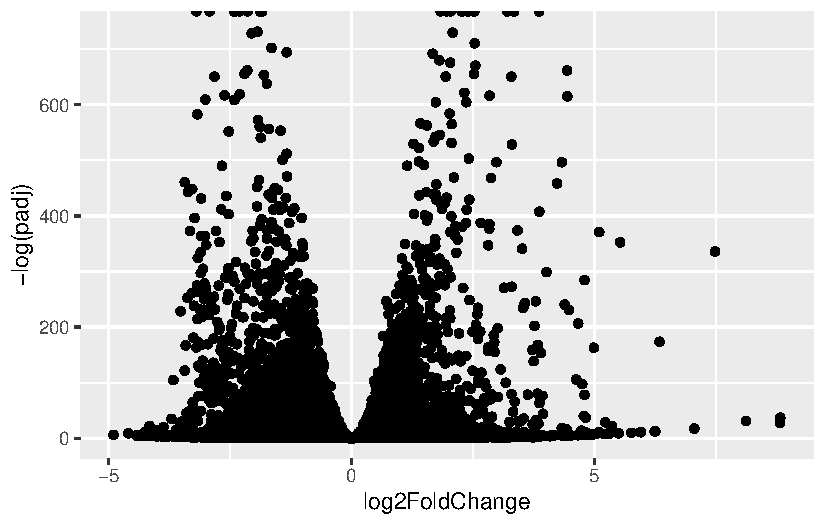
\includegraphics[keepaspectratio]{Class13_files/figure-pdf/unnamed-chunk-9-1.pdf}}

\begin{quote}
Q. Improve this plot by completing the below code, which adds color,
axis labels and cutoff lines:
\end{quote}

\begin{Shaded}
\begin{Highlighting}[]
\NormalTok{mycols }\OtherTok{\textless{}{-}} \FunctionTok{rep}\NormalTok{(}\StringTok{"gray"}\NormalTok{, }\FunctionTok{nrow}\NormalTok{(res))}
\NormalTok{mycols[}\FunctionTok{abs}\NormalTok{(res}\SpecialCharTok{$}\NormalTok{log2FoldChange) }\SpecialCharTok{\textgreater{}} \DecValTok{2}\NormalTok{] }\OtherTok{\textless{}{-}} \StringTok{"blue"}
\NormalTok{mycols[res}\SpecialCharTok{$}\NormalTok{padj }\SpecialCharTok{\textgreater{}} \FloatTok{0.01}\NormalTok{] }\OtherTok{\textless{}{-}} \StringTok{"gray"}

\FunctionTok{ggplot}\NormalTok{(res) }\SpecialCharTok{+}
  \FunctionTok{aes}\NormalTok{(log2FoldChange, }\SpecialCharTok{{-}}\FunctionTok{log}\NormalTok{(padj)) }\SpecialCharTok{+}
  \FunctionTok{geom\_point}\NormalTok{(}\AttributeTok{col=}\NormalTok{mycols) }\SpecialCharTok{+}
  \FunctionTok{xlab}\NormalTok{(}\StringTok{"Log2(FoldChange)"}\NormalTok{) }\SpecialCharTok{+}
  \FunctionTok{ylab}\NormalTok{(}\StringTok{"{-}Log(P{-}value)"}\NormalTok{) }\SpecialCharTok{+}
  \FunctionTok{geom\_vline}\NormalTok{(}\AttributeTok{xintercept=}\FunctionTok{c}\NormalTok{(}\SpecialCharTok{{-}}\DecValTok{2}\NormalTok{, }\DecValTok{2}\NormalTok{)) }\SpecialCharTok{+}
  \FunctionTok{geom\_hline}\NormalTok{(}\AttributeTok{yintercept=}\SpecialCharTok{{-}}\FunctionTok{log}\NormalTok{(}\FloatTok{0.01}\NormalTok{))}
\end{Highlighting}
\end{Shaded}

\begin{verbatim}
Warning: Removed 1237 rows containing missing values or values outside the scale range
(`geom_point()`).
\end{verbatim}

\pandocbounded{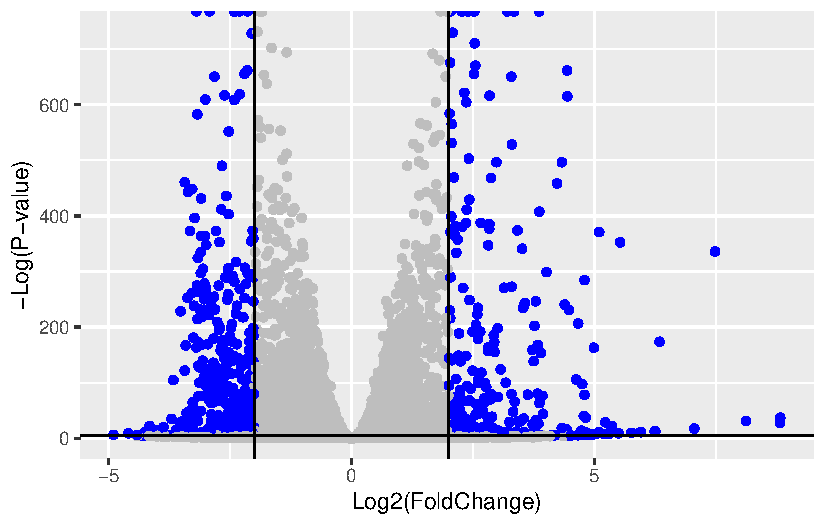
\includegraphics[keepaspectratio]{Class13_files/figure-pdf/unnamed-chunk-10-1.pdf}}

\subsubsection{Adding gene annotation}\label{adding-gene-annotation}

\begin{quote}
Q. Use the mapIDs() function multiple times to add SYMBOL, ENTREZID and
GENENAME annotation to our results by completing the code below.
\end{quote}

\begin{Shaded}
\begin{Highlighting}[]
\FunctionTok{library}\NormalTok{(}\StringTok{"AnnotationDbi"}\NormalTok{)}
\FunctionTok{library}\NormalTok{(}\StringTok{"org.Hs.eg.db"}\NormalTok{)}
\end{Highlighting}
\end{Shaded}

\begin{verbatim}
\end{verbatim}

\begin{Shaded}
\begin{Highlighting}[]
\FunctionTok{columns}\NormalTok{(org.Hs.eg.db)}
\end{Highlighting}
\end{Shaded}

\begin{verbatim}
 [1] "ACCNUM"       "ALIAS"        "ENSEMBL"      "ENSEMBLPROT"  "ENSEMBLTRANS"
 [6] "ENTREZID"     "ENZYME"       "EVIDENCE"     "EVIDENCEALL"  "GENENAME"    
[11] "GENETYPE"     "GO"           "GOALL"        "IPI"          "MAP"         
[16] "OMIM"         "ONTOLOGY"     "ONTOLOGYALL"  "PATH"         "PFAM"        
[21] "PMID"         "PROSITE"      "REFSEQ"       "SYMBOL"       "UCSCKG"      
[26] "UNIPROT"     
\end{verbatim}

\begin{Shaded}
\begin{Highlighting}[]
\NormalTok{res}\SpecialCharTok{$}\NormalTok{symbol }\OtherTok{=} \FunctionTok{mapIds}\NormalTok{(org.Hs.eg.db, }\AttributeTok{keys=}\FunctionTok{row.names}\NormalTok{(res), }\AttributeTok{keytype=}\StringTok{"ENSEMBL"}\NormalTok{,}
                    \AttributeTok{column=}\StringTok{"SYMBOL"}\NormalTok{, }\AttributeTok{multiVals=}\StringTok{"first"}\NormalTok{)}
\end{Highlighting}
\end{Shaded}

\begin{verbatim}
'select()' returned 1:many mapping between keys and columns
\end{verbatim}

\begin{Shaded}
\begin{Highlighting}[]
\NormalTok{res}\SpecialCharTok{$}\NormalTok{entrez }\OtherTok{=} \FunctionTok{mapIds}\NormalTok{(org.Hs.eg.db, }\AttributeTok{keys=}\FunctionTok{row.names}\NormalTok{(res), }\AttributeTok{keytype=}\StringTok{"ENSEMBL"}\NormalTok{,}
                    \AttributeTok{column=}\StringTok{"ENTREZID"}\NormalTok{, }\AttributeTok{multiVals=}\StringTok{"first"}\NormalTok{)}
\end{Highlighting}
\end{Shaded}

\begin{verbatim}
'select()' returned 1:many mapping between keys and columns
\end{verbatim}

\begin{Shaded}
\begin{Highlighting}[]
\NormalTok{res}\SpecialCharTok{$}\NormalTok{name   }\OtherTok{=} \FunctionTok{mapIds}\NormalTok{(org.Hs.eg.db, }\AttributeTok{keys=}\FunctionTok{row.names}\NormalTok{(res), }\AttributeTok{keytype=}\StringTok{"ENSEMBL"}\NormalTok{,}
                    \AttributeTok{column=}\StringTok{"GENENAME"}\NormalTok{, }\AttributeTok{multiVals=}\StringTok{"first"}\NormalTok{)}
\end{Highlighting}
\end{Shaded}

\begin{verbatim}
'select()' returned 1:many mapping between keys and columns
\end{verbatim}

\begin{Shaded}
\begin{Highlighting}[]
\FunctionTok{head}\NormalTok{(res, }\DecValTok{10}\NormalTok{)}
\end{Highlighting}
\end{Shaded}

\begin{verbatim}
log2 fold change (MLE): condition hoxa1 kd vs control sirna 
Wald test p-value: condition hoxa1 kd vs control sirna 
DataFrame with 10 rows and 9 columns
                   baseMean log2FoldChange     lfcSE       stat      pvalue
                  <numeric>      <numeric> <numeric>  <numeric>   <numeric>
ENSG00000279457   29.913579      0.1792571 0.3248215   0.551863 5.81042e-01
ENSG00000187634  183.229650      0.4264571 0.1402658   3.040350 2.36304e-03
ENSG00000188976 1651.188076     -0.6927205 0.0548465 -12.630156 1.43993e-36
ENSG00000187961  209.637938      0.7297556 0.1318599   5.534326 3.12428e-08
ENSG00000187583   47.255123      0.0405765 0.2718928   0.149237 8.81366e-01
ENSG00000187642   11.979750      0.5428105 0.5215598   1.040744 2.97994e-01
ENSG00000188290  108.922128      2.0570638 0.1969053  10.446970 1.51281e-25
ENSG00000187608  350.716868      0.2573837 0.1027266   2.505522 1.22271e-02
ENSG00000188157 9128.439422      0.3899088 0.0467164   8.346302 7.04333e-17
ENSG00000237330    0.158192      0.7859552 4.0804729   0.192614 8.47261e-01
                       padj      symbol      entrez                   name
                  <numeric> <character> <character>            <character>
ENSG00000279457 6.86555e-01          NA          NA                     NA
ENSG00000187634 5.15718e-03      SAMD11      148398 sterile alpha motif ..
ENSG00000188976 1.76553e-35       NOC2L       26155 NOC2 like nucleolar ..
ENSG00000187961 1.13413e-07      KLHL17      339451 kelch like family me..
ENSG00000187583 9.19031e-01     PLEKHN1       84069 pleckstrin homology ..
ENSG00000187642 4.03379e-01       PERM1       84808 PPARGC1 and ESRR ind..
ENSG00000188290 1.30538e-24        HES4       57801 hes family bHLH tran..
ENSG00000187608 2.37452e-02       ISG15        9636 ISG15 ubiquitin like..
ENSG00000188157 4.21970e-16        AGRN      375790                  agrin
ENSG00000237330          NA      RNF223      401934 ring finger protein ..
\end{verbatim}

\begin{quote}
Q. Finally for this section let's reorder these results by adjusted
p-value and save them to a CSV file in your current project directory.
\end{quote}

\begin{Shaded}
\begin{Highlighting}[]
\NormalTok{res }\OtherTok{=}\NormalTok{ res[}\FunctionTok{order}\NormalTok{(res}\SpecialCharTok{$}\NormalTok{pvalue),]}
\FunctionTok{write.csv}\NormalTok{(res, }\AttributeTok{file=}\StringTok{"deseq\_results.csv"}\NormalTok{)}
\end{Highlighting}
\end{Shaded}

\subsection{Pathway Analysis}\label{pathway-analysis}

\begin{Shaded}
\begin{Highlighting}[]
\CommentTok{\# Run in your R console (i.e. not your Rmarkdown doc!)}
\NormalTok{BiocManager}\SpecialCharTok{::}\FunctionTok{install}\NormalTok{( }\FunctionTok{c}\NormalTok{(}\StringTok{"pathview"}\NormalTok{, }\StringTok{"gage"}\NormalTok{, }\StringTok{"gageData"}\NormalTok{) )}
\end{Highlighting}
\end{Shaded}

\begin{verbatim}
Bioconductor version 3.23 (BiocManager 1.30.27), R 4.6.2 (2026-10-29)
\end{verbatim}

\begin{verbatim}
Warning: package(s) not installed when version(s) same as or greater than current; use
  `force = TRUE` to re-install: 'pathview' 'gage' 'gageData'
\end{verbatim}

\begin{verbatim}
Warning in .available.both(repos, method, ...): Some listed binary packages
have no source
\end{verbatim}

\begin{Shaded}
\begin{Highlighting}[]
\CommentTok{\# For old versions of R only (R \textless{} 3.5.0)!}
\CommentTok{\#source("http://bioconductor.org/biocLite.R")}
\CommentTok{\#biocLite( c("pathview", "gage", "gageData") )}
\end{Highlighting}
\end{Shaded}

\begin{Shaded}
\begin{Highlighting}[]
\FunctionTok{library}\NormalTok{(pathview)}
\end{Highlighting}
\end{Shaded}

\begin{verbatim}
##############################################################################
Pathview is an open source software package distributed under GNU General
Public License version 3 (GPLv3). Details of GPLv3 is available at
http://www.gnu.org/licenses/gpl-3.0.html. Particullary, users are required to
formally cite the original Pathview paper (not just mention it) in publications
or products. For details, do citation("pathview") within R.

The pathview downloads and uses KEGG data. Non-academic uses may require a KEGG
license agreement (details at http://www.kegg.jp/kegg/legal.html).
##############################################################################
\end{verbatim}

\begin{Shaded}
\begin{Highlighting}[]
\FunctionTok{library}\NormalTok{(gage)}
\end{Highlighting}
\end{Shaded}

\begin{verbatim}
\end{verbatim}

\begin{Shaded}
\begin{Highlighting}[]
\FunctionTok{library}\NormalTok{(gageData)}

\FunctionTok{data}\NormalTok{(kegg.sets.hs)}
\FunctionTok{data}\NormalTok{(sigmet.idx.hs)}

\CommentTok{\# Focus on signaling and metabolic pathways only}
\NormalTok{kegg.sets.hs }\OtherTok{=}\NormalTok{ kegg.sets.hs[sigmet.idx.hs]}

\CommentTok{\# Examine the first 3 pathways}
\FunctionTok{head}\NormalTok{(kegg.sets.hs, }\DecValTok{3}\NormalTok{)}
\end{Highlighting}
\end{Shaded}

\begin{verbatim}
$`hsa00232 Caffeine metabolism`
[1] "10"   "1544" "1548" "1549" "1553" "7498" "9"   

$`hsa00983 Drug metabolism - other enzymes`
 [1] "10"     "1066"   "10720"  "10941"  "151531" "1548"   "1549"   "1551"  
 [9] "1553"   "1576"   "1577"   "1806"   "1807"   "1890"   "221223" "2990"  
[17] "3251"   "3614"   "3615"   "3704"   "51733"  "54490"  "54575"  "54576" 
[25] "54577"  "54578"  "54579"  "54600"  "54657"  "54658"  "54659"  "54963" 
[33] "574537" "64816"  "7083"   "7084"   "7172"   "7363"   "7364"   "7365"  
[41] "7366"   "7367"   "7371"   "7372"   "7378"   "7498"   "79799"  "83549" 
[49] "8824"   "8833"   "9"      "978"   

$`hsa00230 Purine metabolism`
  [1] "100"    "10201"  "10606"  "10621"  "10622"  "10623"  "107"    "10714" 
  [9] "108"    "10846"  "109"    "111"    "11128"  "11164"  "112"    "113"   
 [17] "114"    "115"    "122481" "122622" "124583" "132"    "158"    "159"   
 [25] "1633"   "171568" "1716"   "196883" "203"    "204"    "205"    "221823"
 [33] "2272"   "22978"  "23649"  "246721" "25885"  "2618"   "26289"  "270"   
 [41] "271"    "27115"  "272"    "2766"   "2977"   "2982"   "2983"   "2984"  
 [49] "2986"   "2987"   "29922"  "3000"   "30833"  "30834"  "318"    "3251"  
 [57] "353"    "3614"   "3615"   "3704"   "377841" "471"    "4830"   "4831"  
 [65] "4832"   "4833"   "4860"   "4881"   "4882"   "4907"   "50484"  "50940" 
 [73] "51082"  "51251"  "51292"  "5136"   "5137"   "5138"   "5139"   "5140"  
 [81] "5141"   "5142"   "5143"   "5144"   "5145"   "5146"   "5147"   "5148"  
 [89] "5149"   "5150"   "5151"   "5152"   "5153"   "5158"   "5167"   "5169"  
 [97] "51728"  "5198"   "5236"   "5313"   "5315"   "53343"  "54107"  "5422"  
[105] "5424"   "5425"   "5426"   "5427"   "5430"   "5431"   "5432"   "5433"  
[113] "5434"   "5435"   "5436"   "5437"   "5438"   "5439"   "5440"   "5441"  
[121] "5471"   "548644" "55276"  "5557"   "5558"   "55703"  "55811"  "55821" 
[129] "5631"   "5634"   "56655"  "56953"  "56985"  "57804"  "58497"  "6240"  
[137] "6241"   "64425"  "646625" "654364" "661"    "7498"   "8382"   "84172" 
[145] "84265"  "84284"  "84618"  "8622"   "8654"   "87178"  "8833"   "9060"  
[153] "9061"   "93034"  "953"    "9533"   "954"    "955"    "956"    "957"   
[161] "9583"   "9615"  
\end{verbatim}

\begin{Shaded}
\begin{Highlighting}[]
\NormalTok{foldchanges }\OtherTok{=}\NormalTok{ res}\SpecialCharTok{$}\NormalTok{log2FoldChange}
\FunctionTok{names}\NormalTok{(foldchanges) }\OtherTok{=}\NormalTok{ res}\SpecialCharTok{$}\NormalTok{entrez}
\FunctionTok{head}\NormalTok{(foldchanges)}
\end{Highlighting}
\end{Shaded}

\begin{verbatim}
     1266     54855      1465      2034      2150      6659 
-2.422719  3.201955 -2.313738 -1.888019  3.344508  2.392288 
\end{verbatim}

\begin{Shaded}
\begin{Highlighting}[]
\CommentTok{\# Get the results}
\NormalTok{keggres }\OtherTok{=} \FunctionTok{gage}\NormalTok{(foldchanges, }\AttributeTok{gsets=}\NormalTok{kegg.sets.hs)}
\end{Highlighting}
\end{Shaded}

\begin{Shaded}
\begin{Highlighting}[]
\FunctionTok{attributes}\NormalTok{(keggres)}
\end{Highlighting}
\end{Shaded}

\begin{verbatim}
$names
[1] "greater" "less"    "stats"  
\end{verbatim}

\begin{Shaded}
\begin{Highlighting}[]
\CommentTok{\# Look at the first few down (less) pathways}
\FunctionTok{head}\NormalTok{(keggres}\SpecialCharTok{$}\NormalTok{less)}
\end{Highlighting}
\end{Shaded}

\begin{verbatim}
                                         p.geomean stat.mean        p.val
hsa04110 Cell cycle                   8.995727e-06 -4.378644 8.995727e-06
hsa03030 DNA replication              9.424076e-05 -3.951803 9.424076e-05
hsa03013 RNA transport                1.375901e-03 -3.028500 1.375901e-03
hsa03440 Homologous recombination     3.066756e-03 -2.852899 3.066756e-03
hsa04114 Oocyte meiosis               3.784520e-03 -2.698128 3.784520e-03
hsa00010 Glycolysis / Gluconeogenesis 8.961413e-03 -2.405398 8.961413e-03
                                            q.val set.size         exp1
hsa04110 Cell cycle                   0.001448312      121 8.995727e-06
hsa03030 DNA replication              0.007586381       36 9.424076e-05
hsa03013 RNA transport                0.073840037      144 1.375901e-03
hsa03440 Homologous recombination     0.121861535       28 3.066756e-03
hsa04114 Oocyte meiosis               0.121861535      102 3.784520e-03
hsa00010 Glycolysis / Gluconeogenesis 0.212222694       53 8.961413e-03
\end{verbatim}

\begin{Shaded}
\begin{Highlighting}[]
\FunctionTok{pathview}\NormalTok{(}\AttributeTok{gene.data=}\NormalTok{foldchanges, }\AttributeTok{pathway.id=}\StringTok{"hsa04110"}\NormalTok{)}
\end{Highlighting}
\end{Shaded}

\begin{verbatim}
'select()' returned 1:1 mapping between keys and columns
\end{verbatim}

\begin{verbatim}
Info: Working in directory /Users/hyuntaean/Desktop/UCSD/BIMM143/R projects BIMM143/Class13
\end{verbatim}

\begin{verbatim}
Info: Writing image file hsa04110.pathview.png
\end{verbatim}

\begin{Shaded}
\begin{Highlighting}[]
\DocumentationTok{\#\# Focus on top 5 upregulated pathways here for demo purposes only}
\NormalTok{keggrespathways }\OtherTok{\textless{}{-}} \FunctionTok{rownames}\NormalTok{(keggres}\SpecialCharTok{$}\NormalTok{greater)[}\DecValTok{1}\SpecialCharTok{:}\DecValTok{5}\NormalTok{]}

\CommentTok{\# Extract the 8 character long IDs part of each string}
\NormalTok{keggresids }\OtherTok{=} \FunctionTok{substr}\NormalTok{(keggrespathways, }\AttributeTok{start=}\DecValTok{1}\NormalTok{, }\AttributeTok{stop=}\DecValTok{8}\NormalTok{)}
\NormalTok{keggresids}
\end{Highlighting}
\end{Shaded}

\begin{verbatim}
[1] "hsa04640" "hsa04630" "hsa00140" "hsa04142" "hsa04330"
\end{verbatim}

\begin{Shaded}
\begin{Highlighting}[]
\FunctionTok{pathview}\NormalTok{(}\AttributeTok{gene.data=}\NormalTok{foldchanges, }\AttributeTok{pathway.id=}\NormalTok{keggresids, }\AttributeTok{species=}\StringTok{"hsa"}\NormalTok{)}
\end{Highlighting}
\end{Shaded}

\begin{verbatim}
'select()' returned 1:1 mapping between keys and columns
\end{verbatim}

\begin{verbatim}
Info: Working in directory /Users/hyuntaean/Desktop/UCSD/BIMM143/R projects BIMM143/Class13
\end{verbatim}

\begin{verbatim}
Info: Writing image file hsa04640.pathview.png
\end{verbatim}

\begin{verbatim}
'select()' returned 1:1 mapping between keys and columns
\end{verbatim}

\begin{verbatim}
Info: Working in directory /Users/hyuntaean/Desktop/UCSD/BIMM143/R projects BIMM143/Class13
\end{verbatim}

\begin{verbatim}
Info: Writing image file hsa04630.pathview.png
\end{verbatim}

\begin{verbatim}
'select()' returned 1:1 mapping between keys and columns
\end{verbatim}

\begin{verbatim}
Info: Working in directory /Users/hyuntaean/Desktop/UCSD/BIMM143/R projects BIMM143/Class13
\end{verbatim}

\begin{verbatim}
Info: Writing image file hsa00140.pathview.png
\end{verbatim}

\begin{verbatim}
'select()' returned 1:1 mapping between keys and columns
\end{verbatim}

\begin{verbatim}
Info: Working in directory /Users/hyuntaean/Desktop/UCSD/BIMM143/R projects BIMM143/Class13
\end{verbatim}

\begin{verbatim}
Info: Writing image file hsa04142.pathview.png
\end{verbatim}

\begin{verbatim}
'select()' returned 1:1 mapping between keys and columns
\end{verbatim}

\begin{verbatim}
Info: Working in directory /Users/hyuntaean/Desktop/UCSD/BIMM143/R projects BIMM143/Class13
\end{verbatim}

\begin{verbatim}
Info: Writing image file hsa04330.pathview.png
\end{verbatim}

\begin{quote}
Q. Can you do the same procedure as above to plot the pathview figures
for the top 5 down-regulated pathways?
\end{quote}

\begin{Shaded}
\begin{Highlighting}[]
\NormalTok{keggrespathways\_down }\OtherTok{\textless{}{-}} \FunctionTok{rownames}\NormalTok{(keggres}\SpecialCharTok{$}\NormalTok{less)[}\DecValTok{1}\SpecialCharTok{:}\DecValTok{5}\NormalTok{]}
\NormalTok{keggresids\_down }\OtherTok{=} \FunctionTok{substr}\NormalTok{(keggrespathways\_down, }\AttributeTok{start=}\DecValTok{1}\NormalTok{, }\AttributeTok{stop=}\DecValTok{8}\NormalTok{)}
\NormalTok{keggresids\_down}
\end{Highlighting}
\end{Shaded}

\begin{verbatim}
[1] "hsa04110" "hsa03030" "hsa03013" "hsa03440" "hsa04114"
\end{verbatim}

\begin{Shaded}
\begin{Highlighting}[]
\DocumentationTok{\#\# "hsa04110" "hsa03030" "hsa03013" "hsa04114" "hsa03440"}

\FunctionTok{pathview}\NormalTok{(}\AttributeTok{gene.data=}\NormalTok{foldchanges, }\AttributeTok{pathway.id=}\NormalTok{keggresids\_down, }\AttributeTok{species=}\StringTok{"hsa"}\NormalTok{)}
\end{Highlighting}
\end{Shaded}

\begin{verbatim}
'select()' returned 1:1 mapping between keys and columns
\end{verbatim}

\begin{verbatim}
Info: Working in directory /Users/hyuntaean/Desktop/UCSD/BIMM143/R projects BIMM143/Class13
\end{verbatim}

\begin{verbatim}
Info: Writing image file hsa04110.pathview.png
\end{verbatim}

\begin{verbatim}
'select()' returned 1:1 mapping between keys and columns
\end{verbatim}

\begin{verbatim}
Info: Working in directory /Users/hyuntaean/Desktop/UCSD/BIMM143/R projects BIMM143/Class13
\end{verbatim}

\begin{verbatim}
Info: Writing image file hsa03030.pathview.png
\end{verbatim}

\begin{verbatim}
'select()' returned 1:1 mapping between keys and columns
\end{verbatim}

\begin{verbatim}
Info: Working in directory /Users/hyuntaean/Desktop/UCSD/BIMM143/R projects BIMM143/Class13
\end{verbatim}

\begin{verbatim}
Info: Writing image file hsa03013.pathview.png
\end{verbatim}

\begin{verbatim}
'select()' returned 1:1 mapping between keys and columns
\end{verbatim}

\begin{verbatim}
Info: Working in directory /Users/hyuntaean/Desktop/UCSD/BIMM143/R projects BIMM143/Class13
\end{verbatim}

\begin{verbatim}
Info: Writing image file hsa03440.pathview.png
\end{verbatim}

\begin{verbatim}
'select()' returned 1:1 mapping between keys and columns
\end{verbatim}

\begin{verbatim}
Info: Working in directory /Users/hyuntaean/Desktop/UCSD/BIMM143/R projects BIMM143/Class13
\end{verbatim}

\begin{verbatim}
Info: Writing image file hsa04114.pathview.png
\end{verbatim}

\subsection{Gene Ontology (GO)}\label{gene-ontology-go}

\begin{Shaded}
\begin{Highlighting}[]
\FunctionTok{data}\NormalTok{(go.sets.hs)}
\FunctionTok{data}\NormalTok{(go.subs.hs)}

\CommentTok{\# Focus on Biological Process subset of GO}
\NormalTok{gobpsets }\OtherTok{=}\NormalTok{ go.sets.hs[go.subs.hs}\SpecialCharTok{$}\NormalTok{BP]}

\NormalTok{gobpres }\OtherTok{=} \FunctionTok{gage}\NormalTok{(foldchanges, }\AttributeTok{gsets=}\NormalTok{gobpsets)}

\FunctionTok{lapply}\NormalTok{(gobpres, head)}
\end{Highlighting}
\end{Shaded}

\begin{verbatim}
$greater
                                             p.geomean stat.mean        p.val
GO:0007156 homophilic cell adhesion       8.519724e-05  3.824205 8.519724e-05
GO:0002009 morphogenesis of an epithelium 1.396681e-04  3.653886 1.396681e-04
GO:0048729 tissue morphogenesis           1.432451e-04  3.643242 1.432451e-04
GO:0007610 behavior                       1.925222e-04  3.565432 1.925222e-04
GO:0060562 epithelial tube morphogenesis  5.932837e-04  3.261376 5.932837e-04
GO:0035295 tube development               5.953254e-04  3.253665 5.953254e-04
                                              q.val set.size         exp1
GO:0007156 homophilic cell adhesion       0.1951953      113 8.519724e-05
GO:0002009 morphogenesis of an epithelium 0.1951953      339 1.396681e-04
GO:0048729 tissue morphogenesis           0.1951953      424 1.432451e-04
GO:0007610 behavior                       0.1967577      426 1.925222e-04
GO:0060562 epithelial tube morphogenesis  0.3565320      257 5.932837e-04
GO:0035295 tube development               0.3565320      391 5.953254e-04

$less
                                            p.geomean stat.mean        p.val
GO:0048285 organelle fission             1.536227e-15 -8.063910 1.536227e-15
GO:0000280 nuclear division              4.286961e-15 -7.939217 4.286961e-15
GO:0007067 mitosis                       4.286961e-15 -7.939217 4.286961e-15
GO:0000087 M phase of mitotic cell cycle 1.169934e-14 -7.797496 1.169934e-14
GO:0007059 chromosome segregation        2.028624e-11 -6.878340 2.028624e-11
GO:0000236 mitotic prometaphase          1.729553e-10 -6.695966 1.729553e-10
                                                q.val set.size         exp1
GO:0048285 organelle fission             5.841698e-12      376 1.536227e-15
GO:0000280 nuclear division              5.841698e-12      352 4.286961e-15
GO:0007067 mitosis                       5.841698e-12      352 4.286961e-15
GO:0000087 M phase of mitotic cell cycle 1.195672e-11      362 1.169934e-14
GO:0007059 chromosome segregation        1.658603e-08      142 2.028624e-11
GO:0000236 mitotic prometaphase          1.178402e-07       84 1.729553e-10

$stats
                                          stat.mean     exp1
GO:0007156 homophilic cell adhesion        3.824205 3.824205
GO:0002009 morphogenesis of an epithelium  3.653886 3.653886
GO:0048729 tissue morphogenesis            3.643242 3.643242
GO:0007610 behavior                        3.565432 3.565432
GO:0060562 epithelial tube morphogenesis   3.261376 3.261376
GO:0035295 tube development                3.253665 3.253665
\end{verbatim}

\subsection{Reactome Analysis}\label{reactome-analysis}

\begin{Shaded}
\begin{Highlighting}[]
\NormalTok{sig\_genes }\OtherTok{\textless{}{-}}\NormalTok{ res[res}\SpecialCharTok{$}\NormalTok{padj }\SpecialCharTok{\textless{}=} \FloatTok{0.05} \SpecialCharTok{\&} \SpecialCharTok{!}\FunctionTok{is.na}\NormalTok{(res}\SpecialCharTok{$}\NormalTok{padj), }\StringTok{"symbol"}\NormalTok{]}
\FunctionTok{print}\NormalTok{(}\FunctionTok{paste}\NormalTok{(}\StringTok{"Total number of significant genes:"}\NormalTok{, }\FunctionTok{length}\NormalTok{(sig\_genes)))}
\end{Highlighting}
\end{Shaded}

\begin{verbatim}
[1] "Total number of significant genes: 8147"
\end{verbatim}

\begin{Shaded}
\begin{Highlighting}[]
\FunctionTok{write.table}\NormalTok{(sig\_genes, }\AttributeTok{file=}\StringTok{"significant\_genes.txt"}\NormalTok{, }\AttributeTok{row.names=}\ConstantTok{FALSE}\NormalTok{, }\AttributeTok{col.names=}\ConstantTok{FALSE}\NormalTok{, }\AttributeTok{quote=}\ConstantTok{FALSE}\NormalTok{)}
\end{Highlighting}
\end{Shaded}

\begin{quote}
Q: What pathway has the most significant ``Entities p-value''? Do the
most significant pathways listed match your previous KEGG results? What
factors could cause differences between the two methods?
\end{quote}

The pathway with the most significant Entities p-value is ``Cell Cycle,
Mitotic'' (p = 1.48E-5, FDR = 2.36E-2), with 407 of its 588 entities
found in our significant gene list. The next most significant pathways
are also all cell-cycle related: Cell Cycle (p = 1.7E-5), Cell Cycle
Checkpoints (p = 4.05E-4), Mitotic Prometaphase (p = 5.81E-4), and
Mitotic Spindle Checkpoint (p = 7.8E-4).

Yes, this matches our KEGG results, where the top down-regulated pathway
was also Cell cycle.

Differences between the two methods can come from:\\
1. Different databases: KEGG and Reactome define pathways differently.
2. Different input: Reactome only used a list of significant genes,
while KEGG/gage used the fold changes of all genes.\\
3. Different statistical tests and gene ID mapping (some genes weren't
recognized).




\end{document}
